\documentclass[11pt,a4paper]{article}
\usepackage{fontspec}
\setmainfont{Source Serif 4}[Path=/home/claude/ref/fonts/, UprightFont=SourceSerif4-Regular.ttf, BoldFont=SourceSerif4-Semibold.ttf, ItalicFont=SourceSerif4-It.ttf]
\setmonofont{IBM Plex Mono}[Path=/home/claude/ref/fonts/, UprightFont=IBMPlexMono-Regular.ttf, BoldFont=IBMPlexMono-Medium.ttf, Scale=0.88]
\usepackage[a4paper,margin=2.4cm]{geometry}
\usepackage{amsmath}
\usepackage{graphicx,booktabs,float,caption,array,xcolor,longtable}
\usepackage{xurl}
\usepackage[hidelinks]{hyperref}
\usepackage[round]{natbib}
\usepackage{setspace}
\setstretch{1.08}
\renewcommand{\topfraction}{0.9}
\renewcommand{\bottomfraction}{0.8}
\renewcommand{\textfraction}{0.1}
\renewcommand{\floatpagefraction}{0.75}
\setlength{\parindent}{0pt}
\setlength{\parskip}{0.55em}
\captionsetup{font=small,labelfont=bf}
\setlength{\bibsep}{3pt}
\urlstyle{same}
\hypersetup{pdftitle={Booth's Poverty Map Today},pdfauthor={Dr Tristan Hotham}}

\begin{document}
\begin{center}
{\Large\bfseries Booth's Poverty Map Today: Street-Level Persistence of Poverty in Inner London, 1898 to 2025\par}
\vspace{1.2em}
{\large Dr Tristan Hotham\par}
\vspace{0.3em}
{\small Independent researcher\\
ORCID: 0000-0003-4931-9349\\
DOI: https://doi.org/10.5281/zenodo.24115200\par}
\vspace{0.8em}
2026
\end{center}

\begin{center}\textbf{Abstract}\end{center}
Charles Booth's map of London poverty records social status street by street, but whether its pattern survives at that scale has rarely been tested. I read the colours of the 1898 to 1899 map automatically along today's OpenStreetMap streets, giving a Booth colour to 19,916 street pieces (2,380~km). On a fresh blind sample labelled by eye by an AI model, the reading agrees exactly for 73\% of judgeable streets and within one step of Booth's seven-step scale for 93\%; it never calls a comfortable street poor but misses many poor ones. Following an analysis pre-specified in a written plan, I compare the share of street in Booth's three poor colours with the Index of Multiple Deprivation 2025 for 1,221 small areas (LSOAs). The rank correlation is 0.20 (95\% CI 0.13 to 0.27); within boroughs, ten percentage points more Booth poverty go with 0.69 more IMD points (CI 0.18 to 1.20), and 0.40 in a spatial error model. The association holds north of the Thames but not south of it, and is local: shifting the historical map by 1~km removes 64\% of it. Street-level persistence of poverty is real but modest; the design is ecological.

\textbf{Keywords:} Charles Booth; poverty; London; historical GIS; persistence; deprivation; map digitisation; Index of Multiple Deprivation

\section{Introduction}

Between 1886 and 1903 Charles Booth's inquiry into \textit{Life and Labour of the People in London} surveyed the social condition of the capital street by street, and its best-known product is a map: every street coloured from black (``Lowest class. Vicious, semi-criminal'') to yellow (``Upper-middle and upper classes. Wealthy''). The revised edition of 1898 to 1899, in twelve sheets, is held by LSE Library, which has digitised it and released the digitised maps under the Creative Commons Public Domain Mark \citep{lse_about, lse_maps}. A georeferenced mosaic of the sheets is served as an overlay by Layers of London, a project whose platform is built by Humap \citep{humap}.

The map invites an obvious question: are the streets Booth coloured poor still the poorer parts of London? The question matters for two reasons. Substantively, a century and a quarter of bombing, slum clearance, council building, deindustrialisation, migration and gentrification separates the two dates, so any surviving association says something about how sticky the social geography of a city is at fine scale. Methodologically, the map is a dense, carefully made record of social status at the level of the individual street, a resolution that modern statistics rarely reach and historical sources almost never do.

This paper makes three contributions. First, it produces an open, reproducible street-level reading of Booth's colours along the modern OpenStreetMap network for the whole of the 1898 to 1899 map, with a blind validation of the reading and a frank account of its errors. Second, it tests, following an analysis plan written before the deprivation data were joined, whether the share of poor streets in each modern small area (LSOA 2021) predicts the English Index of Multiple Deprivation 2025, across the whole map and within boroughs. Third, it asks at what scale any persistence operates, by sliding the historical map away from the areas it describes: if persistence is only the broad contrast between East and West, the correlation should survive a shift of a kilometre or two; if it is local, it should not.

The answer is a modest yes, and a local one. Section~\ref{sec:background} reviews previous work, Section~\ref{sec:data} describes the sources and Section~\ref{sec:measure} the reading of the map. Section~\ref{sec:design} sets out the design, Section~\ref{sec:results} the results and Section~\ref{sec:robust} the planned checks. Section~\ref{sec:discussion} discusses what the findings can and cannot say.

\section{Background}\label{sec:background}

Booth's map is a classification of streets, not of households. Its seven colours summarise the observations of his investigators and should be read as judgements about the predominant character of a street, with mixed streets shown by purple or by combinations of colours \citep{lse_maps}. LSE Library notes that the seven colour codes do not correspond directly to the poverty classes (A to H) of the published survey volumes \citep{lse_maps}. In this paper the colours themselves are the data: black, dark blue and light blue are the three colours of poverty in Booth's legend, purple is ``Mixed. Some comfortable, others poor'', and pink, red and yellow are the comfortable, middle-class and wealthy streets. The legend wording used here is as transcribed by The National Archives \citep{tna}.

\textbf{Previous work.} Booth's material has been set against the present before. \citet{dorling2000} digitised Booth's survey of inner London, aggregated it to 132 wards of 1991 (104 complete and the major part of 28 more) as an index weighting every class by its place in Booth's hierarchy, and found a correlation of 0.73 between that index and a poverty index from the 1991 census; for stomach cancer, stroke and lung cancer, mortality in 1991 to 1995 was predicted more strongly by poverty in 1896 than in 1991. \citet{orford2002} describe the historical GIS behind that work and conclude that the geography of poverty at the end of the nineteenth century was very similar to that at the end of the twentieth. \citet{vaughan2018} places Booth's maps within a longer history of social cartography, from the visual rhetoric of their colours to poverty mapping after Booth, and sets Booth's map of Limehouse beside the IMD 2015; earlier, \citet{vaughan2005} related the colours of East End streets to the configuration of the street network and found the poorest streets more spatially segregated than average. An unpublished master's dissertation \citep{low2019} vectorised eight of the twelve sheets by hand and found that an area-weighted Booth score predicted an index of council tax bands across 2001 MSOAs in a spatial lag model. In economics, \citet{heblich2021} show that the east sides of formerly industrial English cities are more deprived because of neighbourhood sorting that began with historical coal pollution blown east by the prevailing winds, which they estimate explains up to 20\% of neighbourhood segregation in 2011.

The present study differs from this work in four ways: it reads the whole map automatically and openly rather than by hand; it measures along streets, the unit Booth recorded; it uses small areas of about 1,750 residents rather than wards or MSOAs; and it tests directly the spatial scale at which any persistence operates. The comparison with \citet{dorling2000} is instructive: their units were much larger and their index used the whole of Booth's scale, and both differences favour a stronger association than the street-level share of poor colours used here as the main exposure.

\section{Data}\label{sec:data}

\textbf{Booth map.} Web Mercator tiles at zoom 16 (about 1.49~m per pixel at London's latitude) of the georeferenced 1898 to 1899 map as served by Layers of London: 1,535 tiles of 256 pixels covering roughly 0.26$^\circ$W to 0.01$^\circ$E and 51.45$^\circ$N to 51.57$^\circ$N, from Hammersmith and Fulham in the west to Greenwich in the east. The tiles are read in place and are not redistributed; only the derived street colours are.

\textbf{Streets.} OpenStreetMap ways with a road \texttt{highway} tag (residential, primary, secondary, tertiary, trunk, unclassified, pedestrian, living street and links) inside Greater London within the tile box, retrieved from the QLever OSM planet endpoint in 2026 \citep{osm}: 50,010 ways (3,414~km) have their midpoint on the map.

\textbf{Small areas and deprivation.} LSOA 2021 boundaries (generalised, clipped) for the 33 London local authorities from the ONS Open Geography Portal, as packaged in the \texttt{drkane/geo-lookups} repository \citep{geolookups}. The English Indices of Deprivation 2025, File 7, give the IMD score, rank and decile and the domain scores for every LSOA in England \citep{iod2025}. LSOAs average about 1,750 residents in the analysis sample (mid-2022 estimates in the same file).

\section{Reading the map}\label{sec:measure}

\subsection{Inks}
Each pixel is assigned an ``ink'' from its CIELAB colour: paper, grey base-map ink, black, dark blue, light blue, ochre (Booth's yellow), bright red, mauve (Booth's purple prints as a dull mauve) and light red (pink hatching and tints). The thresholds were set by inspecting the map before any deprivation data were joined (\texttt{code/02\_inks.py}).

\subsection{Streets}
Booth coloured house frontages, not the carriageway. Each OSM way is therefore walked every 3 pixels (about 4.5~m), skipping 10 pixels at each end (junctions), and at each position a 7$\times$7-pixel window is read at 5, 7, 9 and 11 pixels (about 7 to 16~m) to each side of the centreline. A window is ``coloured'' if at least 30\% of it is colour ink or at least half is solid black (thin black lettering, boundary dashes and park trees are thereby excluded). The ink counts of all coloured windows along the way are pooled and the street is classified: black if solid black is at least 30\% of the colour ink; otherwise dark or light blue if blue is at least 45\% (dark if dark-blue pixels outnumber light); otherwise yellow if ochre is at least 40\%; otherwise, among the reds, purple if mauve is at least 45\% of the red inks, red if bright red is at least 75\% of bright plus light red, and pink otherwise. A way needs at least four coloured windows to be classified. Figure~\ref{fig:method} shows the reading in Spitalfields.

\begin{figure}[tbp]\centering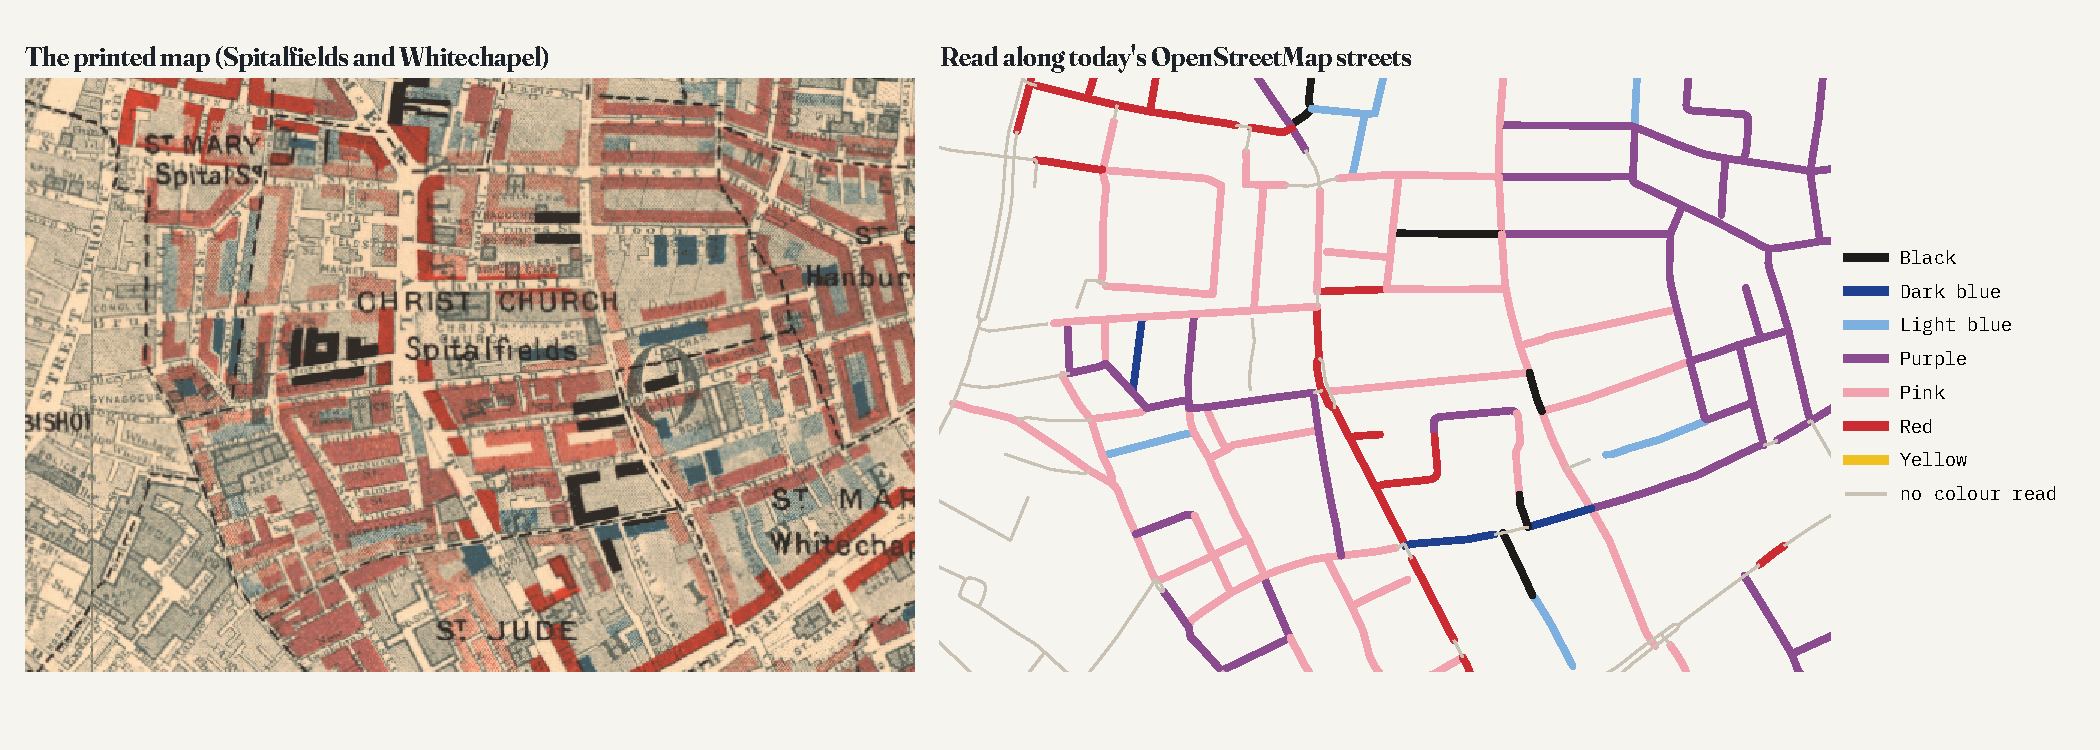
\includegraphics[width=\textwidth]{f_method.pdf}\caption{The printed map (left; LSE Library, Public Domain Mark, via Layers of London) and the colours read along today's OpenStreetMap streets (right) in Spitalfields and Whitechapel. Grey: ways with no colour read.}\label{fig:method}\end{figure}

\subsection{Validation}
A first version of the reader, which took the modal class of individual windows, was checked against 200 randomly drawn coloured ways labelled by eye from magnified crops of the map, blind to the classifier's answer. It agreed exactly for 61\% of judgeable ways and had two systematic faults: narrow solid red frontages read as pink, and thin black lines made some park roads ``black''. The pooled rule above fixed both, before any deprivation data were joined; because this first sample was used to tune the rule it is treated as a development sample (70.8\% exact after the fix). A fresh test sample of 200 coloured ways (excluding all development ways) was then labelled blind. Labels of mixed streets (two colours) count as matches if the reader gives either colour; ways whose colour could not be judged by eye were excluded.

Table~\ref{tab:valid} reports the test sample. Of 200 ways, 23 could not be judged and 23 were mixed. Exact agreement is 73.4\% and agreement within one step of the seven-step scale 93.2\%. For the binary poor/not-poor distinction agreement is 90.4\%: the reader never labelled a non-poor street poor (precision 100\%) but found only 43.3\% of streets with any poor colour, mostly because streets coloured partly purple and partly light blue were read as purple. Among streets with a single poor colour by eye it found 8 of 11. The main confusion elsewhere is between purple and pink, which are hard to separate in the scan. If these errors are unrelated to present deprivation they bias the estimates below towards zero; the misreading of poor streets as purple is not purely random, so this is likely rather than guaranteed. \textbf{The validation labels were made by an AI model} (Claude, Anthropic, the assistant that helped prepare the analysis code), by eye from magnified crops of the map and blind to the reader's output, not by the author or another human coder; the accuracy figures should be read with that in mind (see Section~\ref{sec:discussion}).

\begin{table}[tbp]\centering\small\caption{Test sample: colour by eye (rows) against the reader (columns), ways with a single colour by eye. Mixed ways (23) and ways that could not be judged (23) are not shown.}\label{tab:valid}\begin{tabular}{lrrrrrrrr}\toprule By eye & Black & Dk blue & Lt blue & Purple & Pink & Red & Yellow & Total\\\midrule
Black & 0 & 0 & 0 & 0 & 0 & 0 & 0 & 0\\
Dark blue & 0 & 1 & 0 & 1 & 0 & 0 & 0 & 2\\
Light blue & 0 & 1 & 6 & 0 & 2 & 0 & 0 & 9\\
Purple & 0 & 0 & 0 & 34 & 13 & 5 & 0 & 52\\
Pink & 0 & 0 & 0 & 3 & 28 & 3 & 0 & 34\\
Red & 0 & 0 & 0 & 4 & 6 & 28 & 1 & 39\\
Yellow & 0 & 0 & 0 & 0 & 0 & 2 & 16 & 18\\
\bottomrule\end{tabular}\end{table}

Overall, 19,916 of the 50,010 ways (about 2,380~km) received a colour: 0.4\% of the classified length is black, 3.0\% dark blue, 6.3\% light blue, 23.2\% purple, 36.6\% pink, 21.6\% red and 8.9\% yellow. The share of black is almost certainly too low: much of the black on the map appears to lie on short courts and alleys that are absent from the modern road network.

\section{Design}\label{sec:design}

The analysis was pre-specified in a written plan (\texttt{NOTES.md}) before the deprivation data were joined to the Booth measure; the change to the reader described above was made before that join.

\textbf{Unit.} LSOAs 2021 with at least 90\% of their area on the printed map and at least 300~m of classified street. Of London's 4,994 LSOAs, 1,464 touch the map, 1,310 are at least 90\% covered and 1,221 meet both conditions, in 17 boroughs and 278 MSOAs, with 2,134,501 residents in mid-2022.

\textbf{Exposure.} Booth poverty share: the share of an LSOA's classified street length in black, dark blue or light blue. Ways are split at LSOA boundaries by assigning each sampling position to the LSOA under it, and each piece is classified from its own pooled ink. Its mean in the sample is 10.6\%, and 579 LSOAs have none.

\textbf{Outcome.} The IMD 2025 score (higher is more deprived; sample mean 24.0, standard deviation 10.9).

\textbf{Tests.} (1) Spearman's rank correlation of exposure and outcome, with a 95\% interval from a spatial block bootstrap that resamples 1~km British National Grid squares (205 blocks, 2,000 replicates). (2) OLS of the IMD score on the Booth poverty share (scaled per 10 percentage points) with borough fixed effects and standard errors clustered by MSOA. (3) Moran's $I$ (eight nearest neighbours, row-standardised, 999 permutations) of the exposure, the outcome and the residuals of model 2; because the residuals proved spatially autocorrelated, the planned spatial error model with borough dummies (maximum likelihood, \texttt{spreg}) is also reported.

\textbf{Planned robustness.} Purple counted as poor; Booth's mean score on a 1 (black) to 7 (yellow) scale; the share of all poor-ink map area in the LSOA rather than street length; only street pieces with purity at least 0.6; a stricter sample (fully covered, at least 500~m classified); the income domain score and the national IMD rank as outcomes; leaving out each borough with at least 20 LSOAs; north and south of the Thames separately; and without the City of London.

\textbf{Scale test.} Every LSOA polygon is shifted by 500~m, 1, 2 and 4~km in eight directions, and the Booth measure re-read under the shifted polygon while the outcome stays the LSOA's own score. If persistence is local, the association should fall quickly with distance.

\textbf{What would count against persistence.} A rank correlation whose interval includes zero, or a within-borough coefficient near zero.

\section{Results}\label{sec:results}

Figure~\ref{fig:map} sets the two maps side by side. Booth's yellow is concentrated west of the City, in Mayfair, Belgravia, Kensington and Bayswater; blue streets are scattered more widely, with more of them east of the City and south of the river. Today's deprivation is highest in the north-east and north-west of the study area.

\begin{figure}[tbp]\centering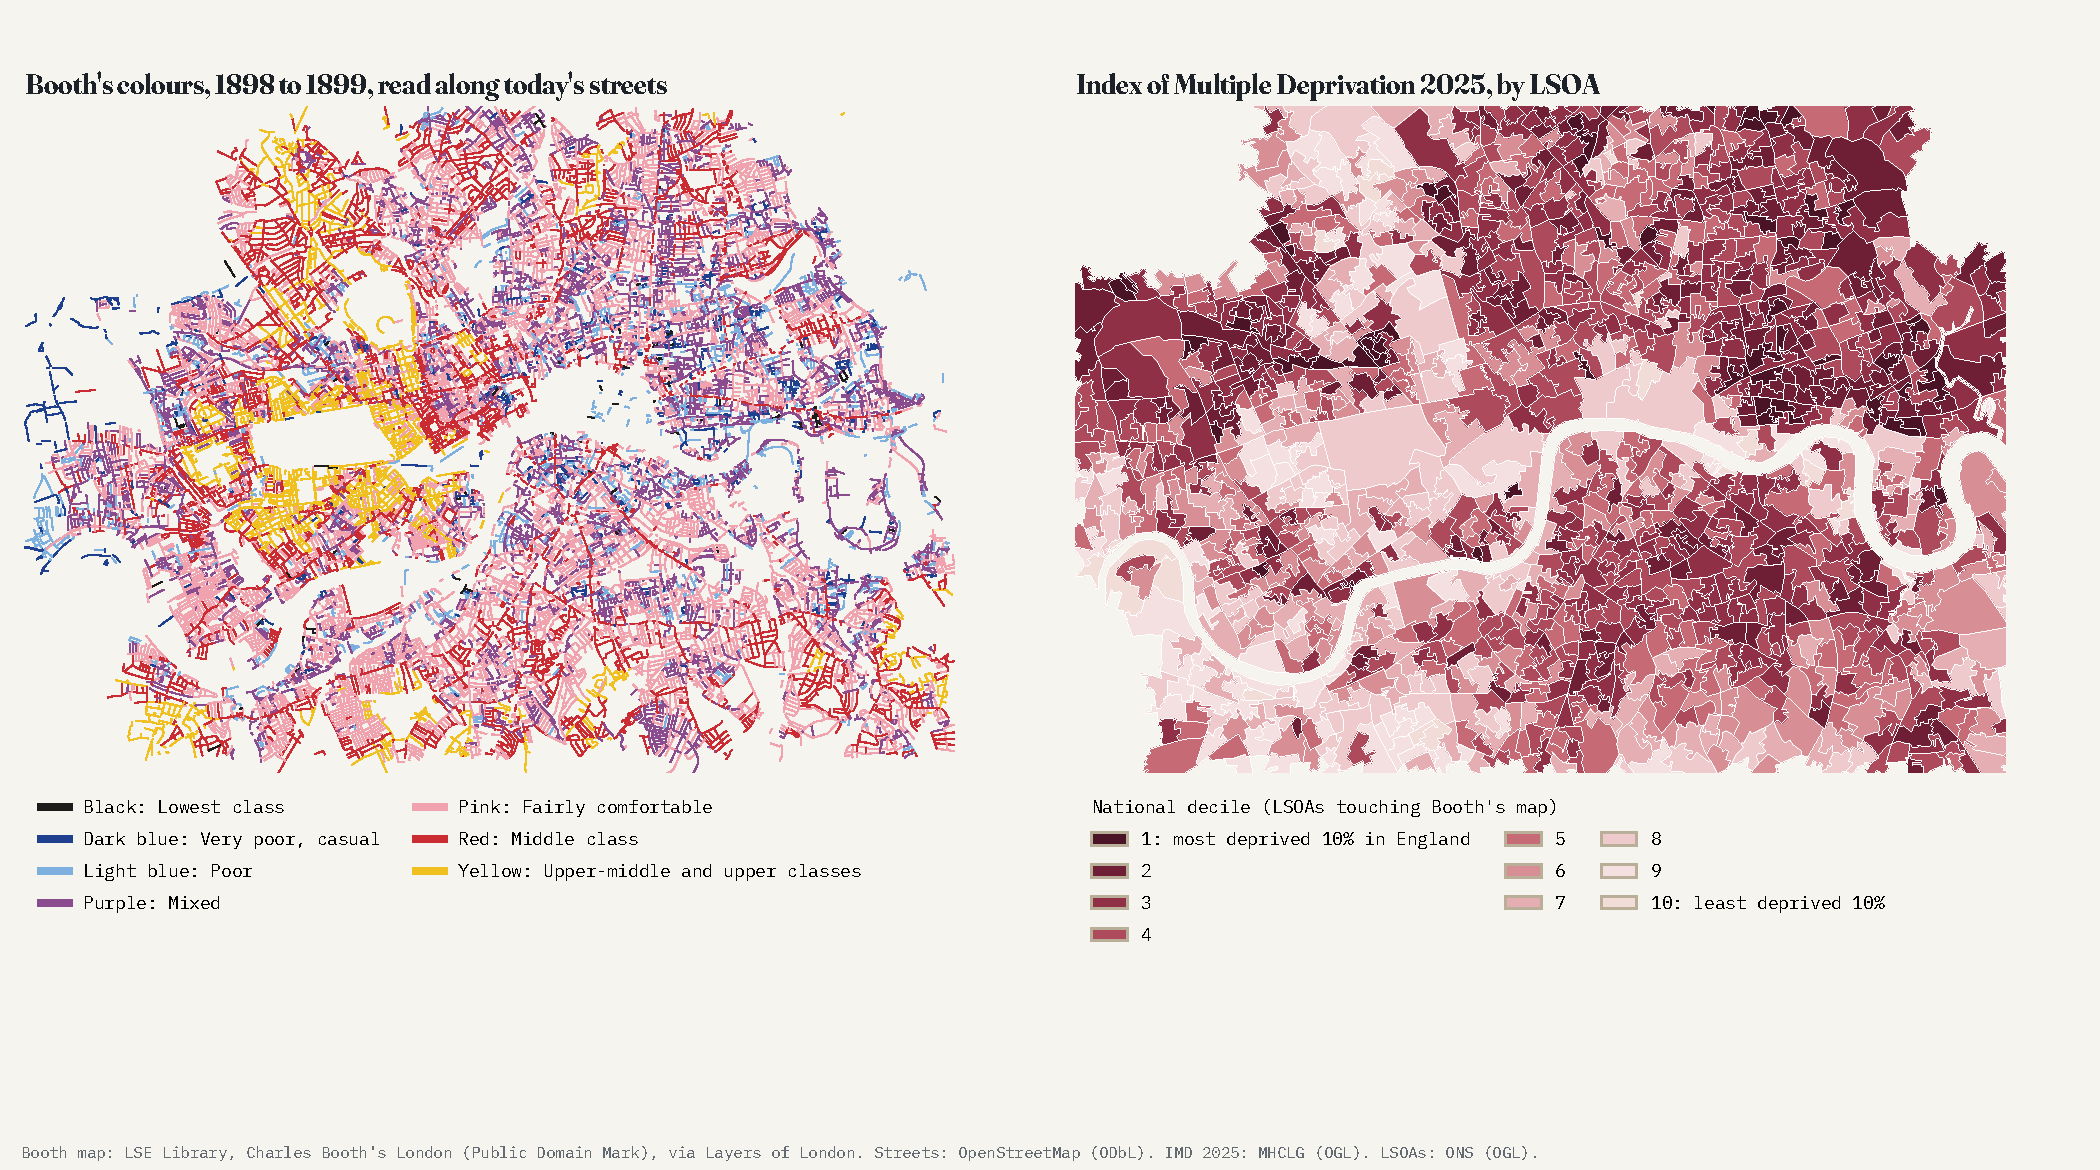
\includegraphics[width=\textwidth]{f_map.pdf}\caption{Left: Booth's colours (1898 to 1899) read along today's streets. Right: IMD 2025 national deciles by LSOA for the LSOAs touching the map.}\label{fig:map}\end{figure}

The main estimates are in Table~\ref{tab:main}. The rank correlation between Booth poverty share and the IMD 2025 score is 0.20 (95\% CI 0.13 to 0.27; $N=1,221$). Within boroughs, ten percentage points of Booth poverty go with 0.69 more IMD points (CI 0.18 to 1.20, $p=0.008$); without borough effects the slope is 0.81 (CI 0.25 to 1.36). Moving from no poor streets to all poor streets is thus associated with about 6.9 IMD points, 0.63 of a standard deviation of the sample's scores. The exposure explains little of the outcome on its own ($R^2=0.017$).

\begin{table}[tbp]\centering\small\caption{Main estimates. Outcome: IMD 2025 score. Exposure: Booth poverty share (black, dark blue, light blue) per 10 percentage points. (1) Spearman rank correlation, 95\% interval from a 1~km block bootstrap (2,000 replicates). (2) OLS without and (3) with borough fixed effects, standard errors clustered by MSOA. (4) Spatial error model with borough dummies, 8 nearest neighbours.}\label{tab:main}\resizebox{\textwidth}{!}{\begin{tabular}{lrrrr}\toprule & (1) Spearman & (2) OLS & (3) OLS, borough FE & (4) Spatial error\\\midrule
Estimate & 0.203 & 0.807 & 0.688 & 0.404\\
95\% interval & [0.134, 0.267] & [0.251, 1.363] & [0.178, 1.198] & [0.070, 0.738]\\
Standardised outcome & & & 0.063 [0.016, 0.110] & \\
$R^2$ & & 0.017 & 0.191 & \\
$\lambda$ & & & & 0.644\\
N (LSOAs) & 1,221 & 1,221 & 1,221 & 1,221\\
Clusters (MSOAs) / boroughs & & 278 & 278 / 17 & \\\bottomrule\end{tabular}}\end{table}

Both measures are strongly clustered in space (Moran's $I$ 0.30 for the Booth share and 0.41 for the IMD), and so are the residuals of model 2 (0.28). In the spatial error model the within-borough slope falls to 0.40 (CI 0.07 to 0.74) with a spatial parameter $\lambda=0.64$: some of the simple association is shared neighbourhood context, but not all of it.

Figure~\ref{fig:ends} shows the association across the range of Booth poverty and, for comparison, for the share of street that Booth coloured red or yellow. The relation for the poor colours is shallow and noisy; the relation for the wealthy colours is steeper and more regular. In an exploratory analysis not in the plan, the share of red and yellow street correlates with the IMD at -0.36 (CI -0.42 to -0.29), and the yellow share alone at -0.37. Of the 74 LSOAs where at least half of the classified street was yellow, 34 are in national IMD deciles 8 to 10 and 4 in deciles 1 or 2.

\begin{figure}[tbp]\centering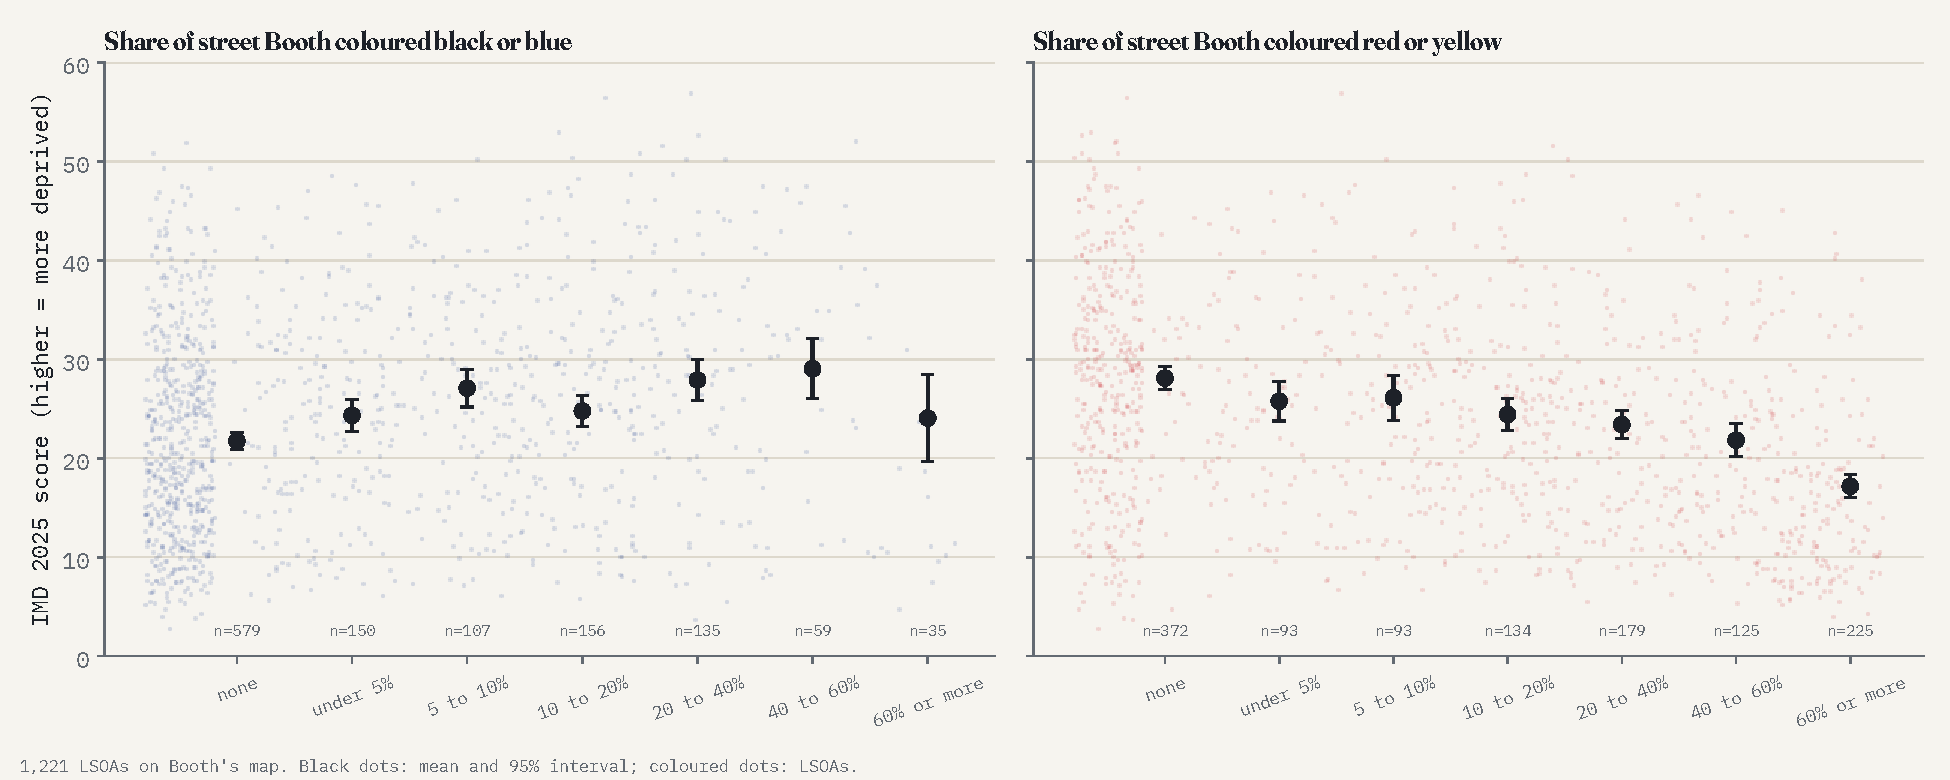
\includegraphics[width=\textwidth]{f_ends.pdf}\caption{IMD 2025 score by bands of the share of an LSOA's classified street that Booth coloured black or blue (left, the planned exposure) and red or yellow (right, exploratory). Means with 95\% intervals; dots are LSOAs.}\label{fig:ends}\end{figure}

Table~\ref{tab:cross} and Figure~\ref{fig:cross} cross-tabulate Booth poverty groups with national IMD deciles. The planned quintiles could not be formed because 579 LSOAs (579 in all) have no poor street at all; group 1 is these LSOAs and groups 2 to 5 are quartiles of the rest. The mean IMD score is 21.8 in group 1 and 27.6 in group 5, but groups 3 to 5 differ little, and the share of LSOAs in the most deprived fifth of England rises from 13.3\% to 31.7\%.

\begin{table}[tbp]\centering\small\caption{LSOAs by Booth poverty group (1 = no poor street; 2 to 5 = quartiles of the rest) and national IMD 2025 decile (1 = most deprived), with the mean IMD score.}\label{tab:cross}\begin{tabular}{lrrrrrrrrrrrr}\toprule Group & 1 & 2 & 3 & 4 & 5 & 6 & 7 & 8 & 9 & 10 & N & Mean IMD\\\midrule
1 & 12 & 65 & 98 & 93 & 83 & 80 & 56 & 49 & 35 & 8 & 579 & 21.8\\
2 & 5 & 27 & 38 & 25 & 22 & 14 & 8 & 14 & 8 & 0 & 161 & 24.5\\
3 & 6 & 34 & 37 & 31 & 17 & 16 & 6 & 6 & 7 & 0 & 160 & 26.3\\
4 & 10 & 25 & 38 & 33 & 14 & 12 & 13 & 10 & 5 & 0 & 160 & 26.0\\
5 & 16 & 35 & 35 & 21 & 16 & 6 & 9 & 15 & 5 & 3 & 161 & 27.6\\
\bottomrule\end{tabular}\end{table}

\begin{figure}[tbp]\centering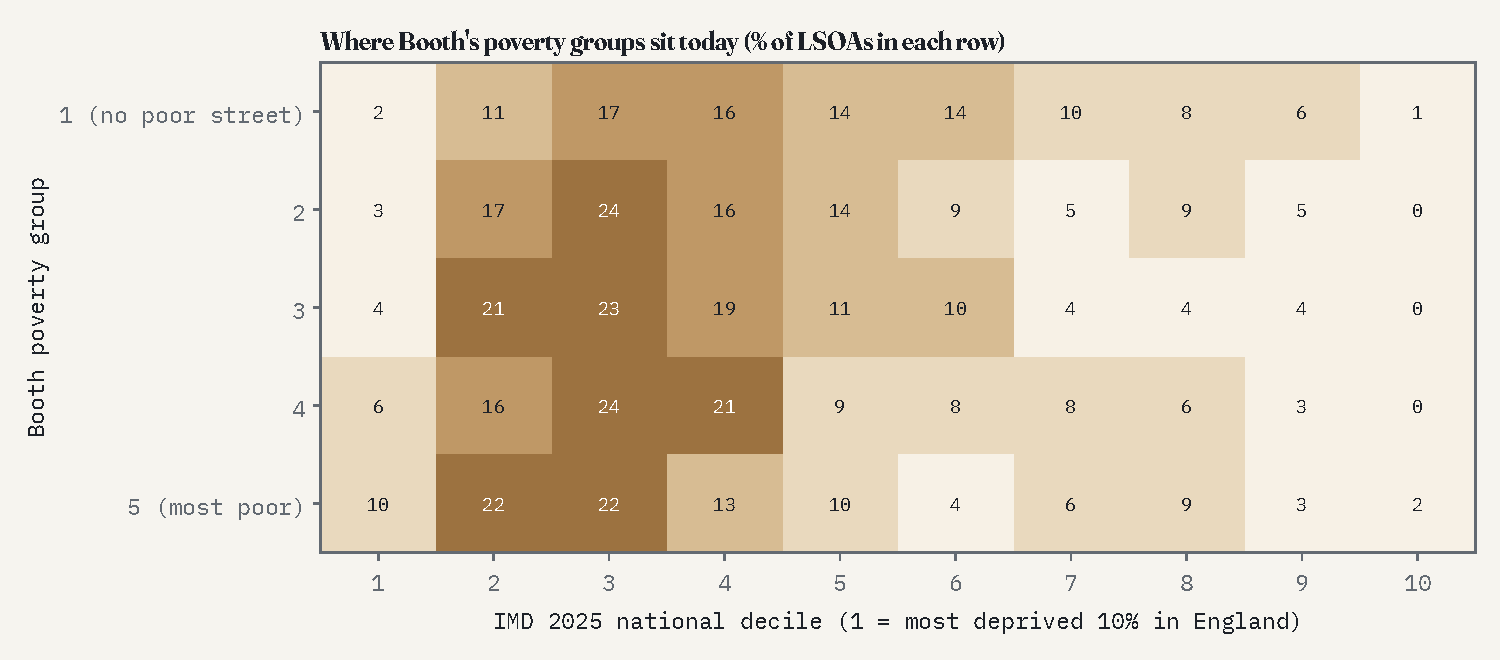
\includegraphics[width=0.85\textwidth]{f_crosstab.pdf}\caption{Percentage of LSOAs in each Booth poverty group (rows; 1 = no poor street, 2 to 5 = quartiles of the rest) by national IMD 2025 decile (columns).}\label{fig:cross}\end{figure}

\textbf{Persistent, turned around and fallen.} Defining Booth's poorest fifth as the 244 LSOAs with the highest poverty share (at least 18.9\% of coloured street), 72 of them are in IMD deciles 1 or 2 today; 32 of them are in Tower Hamlets. 58 of the poorest fifth are now in deciles 6 to 10, many along the Thames (Rotherhithe, Nine Elms, Sands End, Putney). 77 LSOAs with no poor street at all on Booth's map are now in deciles 1 or 2, 39 of them in Hackney, Islington and Camden (Figure~\ref{fig:groups}). Neighbourhood names are the nearest Wikidata area, suburb or neighbourhood point within 1.5~km.

\begin{figure}[tbp]\centering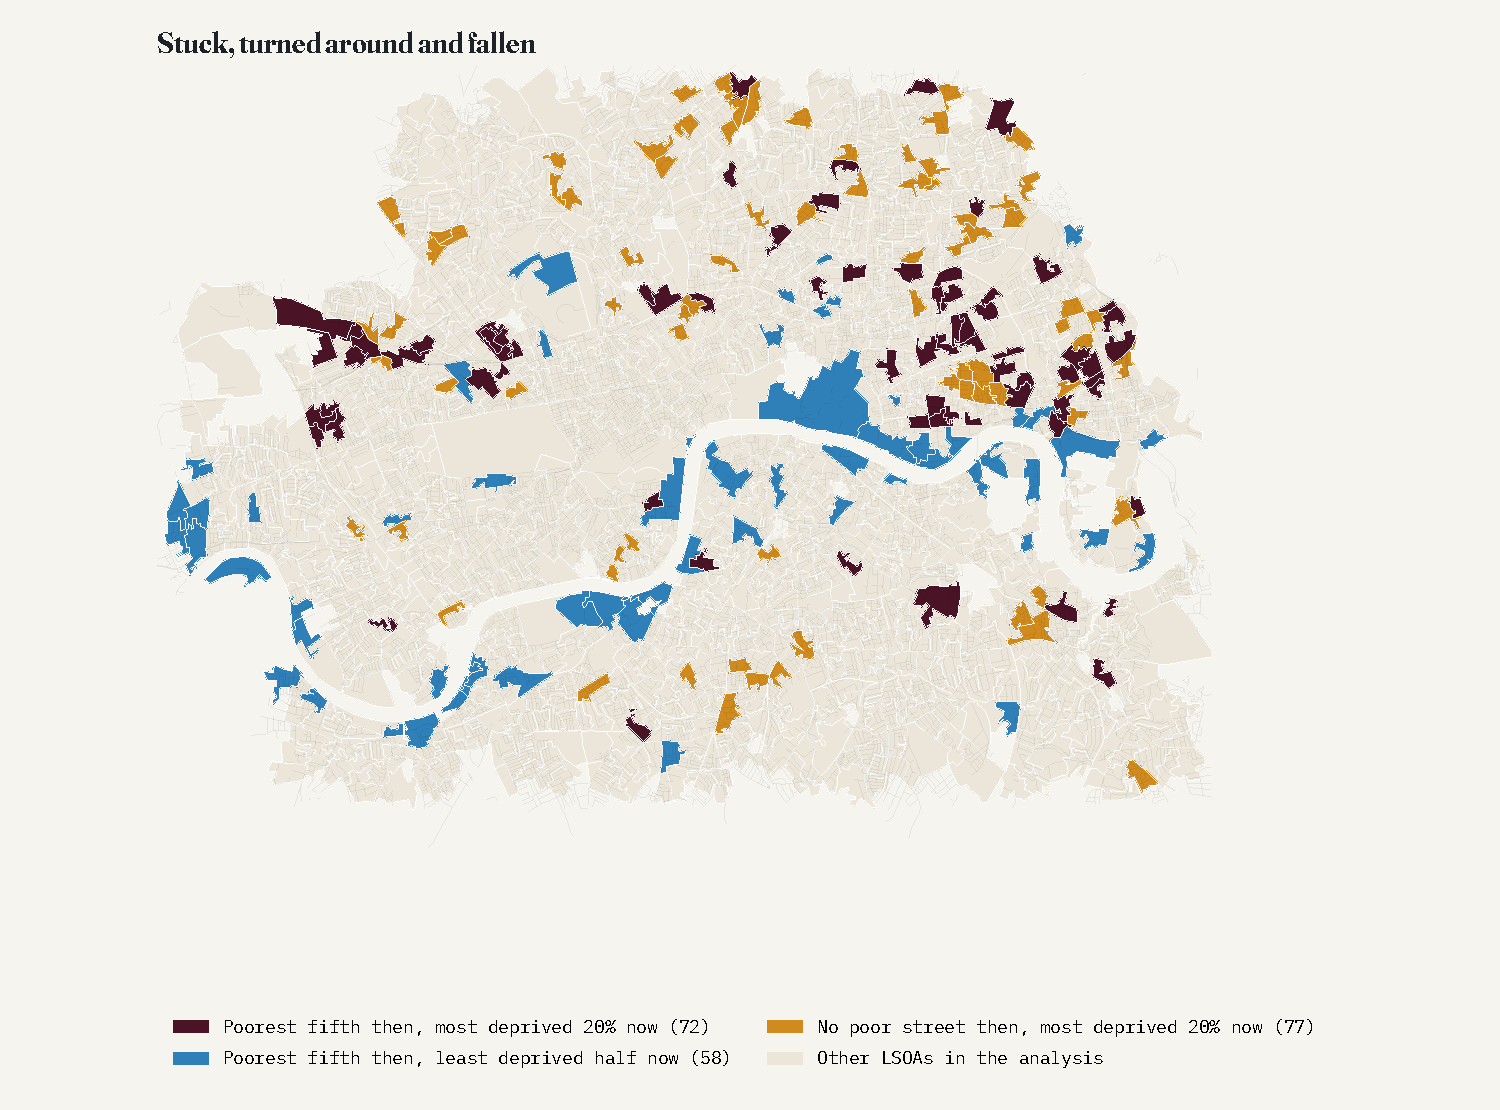
\includegraphics[width=0.85\textwidth]{f_groups.pdf}\caption{Persistent (Booth's poorest fifth, IMD deciles 1 or 2), turned around (poorest fifth, deciles 6 to 10) and fallen (no poor street on Booth's map, deciles 1 or 2) LSOAs.}\label{fig:groups}\end{figure}

\section{Robustness}\label{sec:robust}

Table~\ref{tab:robust} and Figure~\ref{fig:robust} report the planned checks. Counting purple as poor strengthens the association (rho 0.33), and Booth's seven-step mean score correlates with the IMD at -0.37 (negative because higher scores mean wealthier). Using map area rather than street length, keeping only high-purity streets, or a stricter sample gives correlations from 0.17 to 0.24; across all seven planned variants of the exposure and sample (R1, R3 to R5, R8a to R8c) the range is 0.09 (south of the Thames) to 0.33 (purple counted as poor). Leaving out each of the 11 boroughs with at least 20 LSOAs gives correlations from 0.17 to 0.21 and within-borough slopes from 0.48 to 1.20. The income domain and the national IMD rank give similar results.

The planned split by the Thames matters. North of the river the correlation is 0.25 (CI 0.17 to 0.32, $N=809$); south of it, 0.09 (CI -0.03 to 0.21, $N=412$), and the within-borough slope is 0.20 (CI -0.37 to 0.76). The persistence found here is therefore a north-of-the-river result; I do not claim it for south London.

\begin{table}[tbp]\centering\footnotesize\caption{Planned robustness checks. Spearman correlation (500 block-bootstrap replicates) and within-borough OLS slope (per 10 percentage points of the exposure, or per point of the mean score; R6a in income-domain units, R6b in national rank places), 95\% intervals.}\label{tab:robust}\begin{tabular}{p{6.2cm}rll}\toprule Check & N & Spearman & Borough FE slope\\\midrule
Main specification & 1,221 & 0.203 [0.134, 0.267] & 0.688 [0.178, 1.198]\\
R1 purple counted as poor & 1,221 & 0.334 [0.267, 0.403] & 0.928 [0.628, 1.228]\\
R2 mean Booth score (1 black to 7 yellow) & 1,221 & -0.373 [-0.435, -0.293] & -4.480 [-5.636, -3.325]\\
R3 map area instead of streets & 1,221 & 0.165 [0.087, 0.240] & 0.631 [0.147, 1.116]\\
R4 streets with purity at least 0.6 & 1,217 & 0.188 [0.108, 0.251] & 0.700 [0.152, 1.247]\\
R5 fully covered, at least 500 m classified & 1,135 & 0.238 [0.160, 0.307] & 1.076 [0.513, 1.638]\\
R6a income domain score & 1,221 & 0.243 [0.176, 0.308] & 0.011 [0.004, 0.018]\\
R6b IMD national rank (most deprived high) & 1,221 & 0.203 [0.130, 0.268] & 371.984 [48.880, 695.089]\\
R8a north of the Thames & 809 & 0.247 [0.168, 0.324] & 0.893 [0.218, 1.568]\\
R8b south of the Thames & 412 & 0.093 [-0.026, 0.213] & 0.195 [-0.367, 0.757]\\
R8c without the City of London & 1,218 & 0.205 [0.133, 0.268] & 0.700 [0.182, 1.217]\\
Window-mode classifier (first version) (not planned) & 1,221 & 0.194 [0.127, 0.254] & 0.609 [0.088, 1.129]\\
\bottomrule\end{tabular}\end{table}

\begin{figure}[tbp]\centering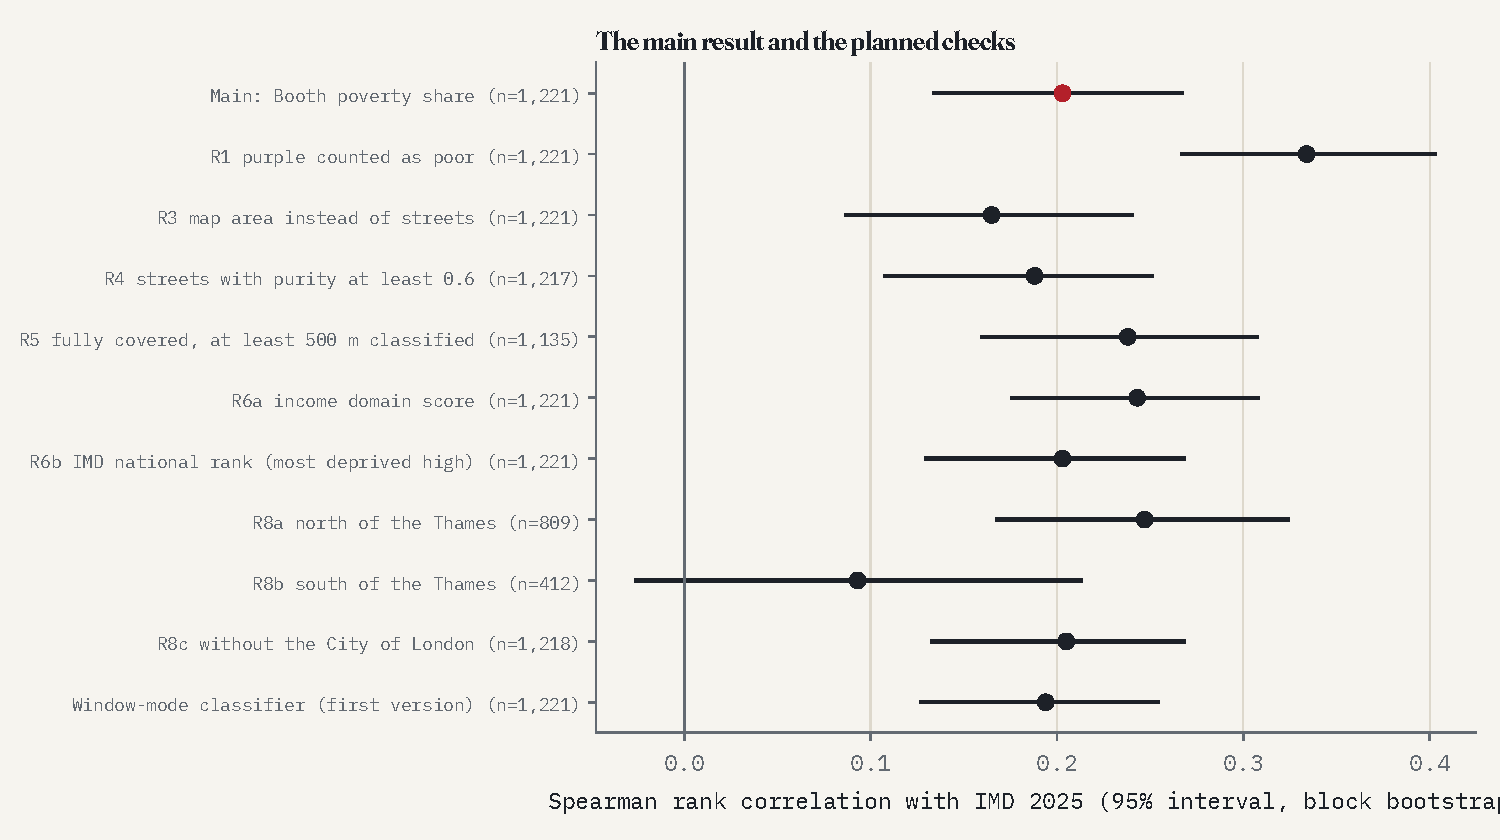
\includegraphics[width=0.85\textwidth]{f_robust.pdf}\caption{Spearman correlations with the IMD 2025 score for the main specification and the planned checks (95\% spatial block-bootstrap intervals; 500 replicates for the checks).}\label{fig:robust}\end{figure}

\textbf{Scale.} Figure~\ref{fig:shift} and Table~\ref{tab:shift} show the scale test. Shifting the historical map by 500~m lowers the mean correlation from 0.20 to 0.12; at 1~km it is 0.07 and at 2~km 0.02, with directional values straddling zero. The within-borough slope falls in step. Persistence is therefore local: what survives is the contrast between neighbouring streets and blocks, not only the broad contrast between East and West.

\begin{table}[tbp]\centering\small\caption{Scale test: LSOAs shifted in eight directions; mean and range over directions of the Spearman correlation and of the within-borough slope.}\label{tab:shift}\begin{tabular}{lrrlrl}\toprule Shift & Mean N & Mean rho & Range & Mean slope & Range\\\midrule
None & 1,221 & 0.203 & [0.203, 0.203] & 0.688 & [0.688, 0.688]\\
500 m & 1,158 & 0.124 & [0.094, 0.173] & 0.368 & [0.197, 0.577]\\
1 km & 1,103 & 0.074 & [0.047, 0.105] & 0.187 & [-0.092, 0.354]\\
2 km & 1,044 & 0.021 & [-0.065, 0.089] & 0.117 & [-0.184, 0.454]\\
4 km & 975 & 0.019 & [-0.160, 0.112] & -0.025 & [-0.534, 0.641]\\
\bottomrule\end{tabular}\end{table}

\begin{figure}[tbp]\centering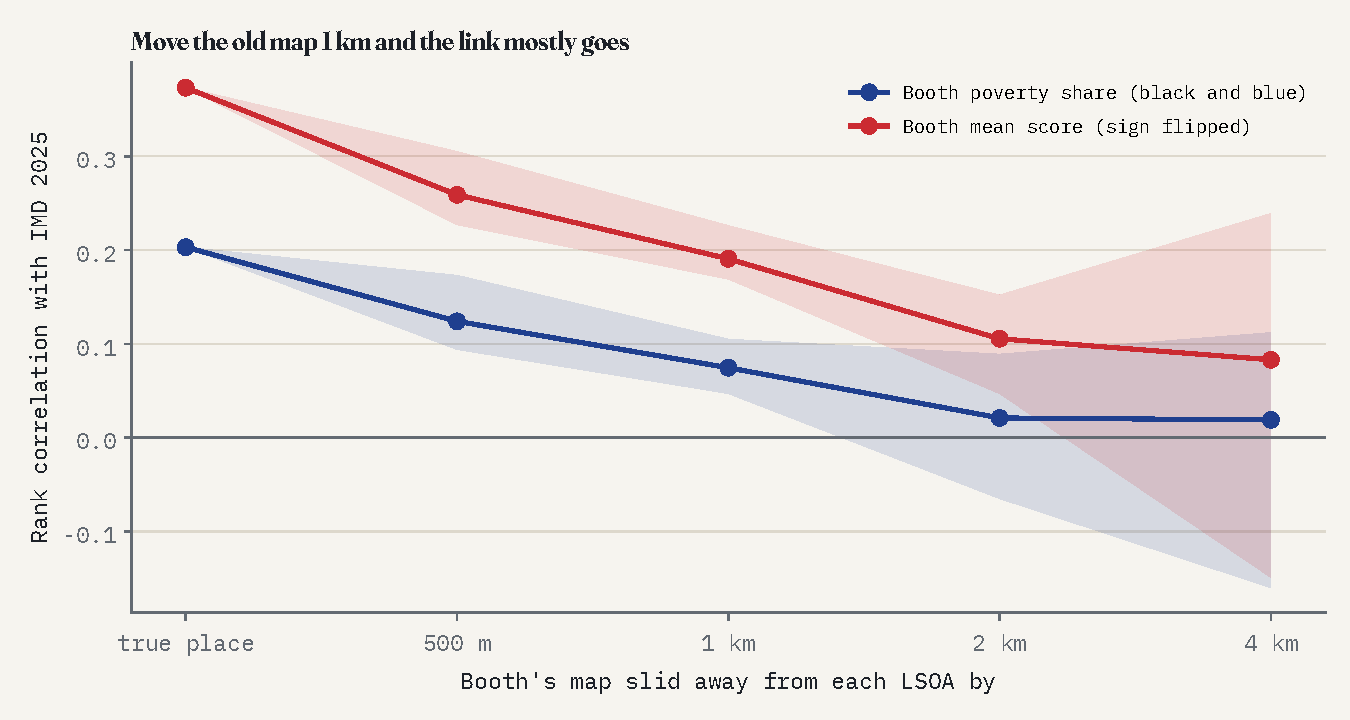
\includegraphics[width=0.75\textwidth]{f_shift.pdf}\caption{Rank correlation between the Booth measure read under each LSOA shifted by the given distance (mean over eight directions; shaded, range) and the LSOA's own IMD 2025 score.}\label{fig:shift}\end{figure}

\section{Discussion}\label{sec:discussion}

Read at street level and compared with the IMD 2025, Booth's 1898 to 1899 map retains a modest, local and mainly north-of-the-river association with deprivation today. The planned test favours persistence, but the effect is small relative to the variation in today's deprivation, and it weakens once spatial clustering is modelled. The full seven-step scale, and especially its wealthy end, is more strongly associated with present deprivation than the poor colours alone; this was not part of the plan and should be tested further rather than taken as a finding.

Several limitations qualify these results. (i) The design is ecological and correlational: it compares places, not people, and says nothing about the descendants of Booth's families or about mechanisms. Between the two maps lie the Blitz, slum clearance, council building, the closure of the docks and decades of housing-market change; any of these could create, break or preserve associations. (ii) The reading of the map is imperfect: it under-detects poor streets, particularly mixed purple and light blue ones, and confuses purple with pink. Errors that are unrelated to present deprivation bias estimates towards zero. The validation labels were made by an AI model (Claude) by eye from magnified crops, blind to the classifier's output; no human coder has yet labelled the sample, and an independent human labelling would strengthen the paper. (iii) Short courts and alleys, often the poorest places on Booth's map, are under-represented because they are absent from the modern road network. (iv) The IMD is a relative index of 2020s indicators, not a measure of the same thing Booth recorded. (v) The study covers the area of the 1898 to 1899 map only.

\section{Conclusion}\label{sec:conclusion}

An automated, validated reading of Charles Booth's poverty map along today's streets shows that the poorer streets of the 1890s are, on average, slightly more deprived in 2025, within boroughs as well as across them, north of the Thames, and only at a very local scale. The street-level data and code are released openly so that the reading can be improved, re-validated and linked to other outcomes.

\section*{Data availability}
Data and code: Zenodo DOI https://doi.org/10.5281/zenodo.24115200; also \url{https://github.com/Tristan-Hotham/booth-today}. The derived street classification (\texttt{data/streets\_booth.csv.gz}) is derived from OpenStreetMap and shared under the ODbL; the LSOA-level data and all other derived files are CC~BY~4.0. The Booth map tiles are not redistributed; they are available from LSE Library and Layers of London.

\section*{AI statement}
I wrote the text, with drafting and editing assistance from Claude (Anthropic), which also helped prepare the analysis code. I reviewed and checked all text and results.

\bibliographystyle{plainnat}
\begin{thebibliography}{99}\small
\bibitem[Humap(2026)]{humap} Humap (2026) Charles Booth's London (case study). \url{https://humap.me/case-studies/charles-booths-london/} (accessed 2026).
\bibitem[Dorling et~al.(2000)]{dorling2000} Dorling, D., Mitchell, R., Shaw, M., Orford, S. and Davey Smith, G. (2000) The ghost of Christmas past: health effects of poverty in London in 1896 and 1991. \textit{BMJ} 321(7276), 1547--1551. \url{https://doi.org/10.1136/bmj.321.7276.1547}
\bibitem[Heblich et~al.(2021)]{heblich2021} Heblich, S., Trew, A. and Zylberberg, Y. (2021) East-side story: historical pollution and persistent neighborhood sorting. \textit{Journal of Political Economy} 129(5), 1508--1552. \url{https://doi.org/10.1086/713101}
\bibitem[drkane(2026)]{geolookups} Kane, D. (2026) geo-lookups: a collection of data resources for handling small-area UK geography. GitHub repository \url{https://github.com/drkane/geo-lookups}; boundaries from the ONS Open Geography Portal (Open Government Licence v3.0).
\bibitem[LSE Library(2026a)]{lse_about} LSE Library (2026a) Charles Booth's London: About. \url{https://booth.lse.ac.uk/about} (accessed 2026).
\bibitem[LSE Library(2026b)]{lse_maps} LSE Library (2026b) What were the poverty maps? Charles Booth's London. \url{https://booth.lse.ac.uk/learn-more/what-were-the-poverty-maps} (accessed 2026).
\bibitem[Low(2019)]{low2019} Low, W. D. (2019) Charles Booth's poverty maps and modern patterns of affluence: understanding their relationship through vectorisation and spatial regression. MSc dissertation, Centre for Advanced Spatial Analysis, University College London (unpublished). \url{https://williamlow.github.io/Booth_poverty/booth-poverty-modern-patterns.html}
\bibitem[MHCLG(2025)]{iod2025} Ministry of Housing, Communities and Local Government (2025) English Indices of Deprivation 2025, File 7: all ranks, scores, deciles and population denominators. Open Government Licence v3.0.
\bibitem[Orford et~al.(2002)]{orford2002} Orford, S., Dorling, D., Mitchell, R., Shaw, M. and Davey Smith, G. (2002) Life and death of the people of London: a historical GIS of Charles Booth's inquiry. \textit{Health and Place} 8(1), 25--35. \url{https://doi.org/10.1016/S1353-8292(01)00033-8}
\bibitem[OpenStreetMap contributors(2026)]{osm} OpenStreetMap contributors (2026) OpenStreetMap, retrieved via the QLever OSM planet endpoint. Open Database Licence.
\bibitem[The National Archives(2026)]{tna} The National Archives (2026) Charles Booth's poverty map of London (Archives Live: Whitechapel education resource). \url{https://www.nationalarchives.gov.uk/education/resources/archives-live-whitechapel/archives-live-whitechapel-charles-booth-map/} (accessed 2026).
\bibitem[Vaughan et~al.(2005)]{vaughan2005} Vaughan, L., Clark, D. C. and Sahbaz, O. (2005) Space and exclusion: the relationship between physical segregation, economic marginalisation and poverty in the city. Paper presented to the Fifth International Space Syntax Symposium, Delft.
\bibitem[Vaughan(2018)]{vaughan2018} Vaughan, L. (2018) \textit{Mapping Society: The Spatial Dimensions of Social Cartography}. London: UCL Press (open access, CC BY-NC-ND 4.0). \url{https://doi.org/10.14324/111.9781787353053}
\end{thebibliography}

\appendix
\section{Data construction details}
\label{app:data}
\sloppy
The classification palette (every colour of the tiles with its ink) is \texttt{data/ink\_palette.csv}. Per-way pooled ink counts, colour, purity and the first-version (window mode) colour are in \texttt{data/streets\_booth.csv.gz}; per-LSOA measures in \texttt{data/lsoa\_booth.csv} and the analysis sample in \texttt{data/lsoa\_analysis.csv}. Validation labels and scores are in \texttt{code/validation\_dev\_labels.csv}, \texttt{code/validation\_test\_labels.csv} and \texttt{data/validation\_*.json}. The full model output is \texttt{data/models.json} and the scale test \texttt{data/shift.json}. The first-version reader, used as a robustness check, gives rho 0.19 (CI 0.13 to 0.25).

\end{document}
